\documentclass[12pt]{beamer}
\usepackage{verbatim}
\usepackage{ifthen}

\usepackage{tikz}
\usetikzlibrary{arrows, positioning}
\usepackage{pgfplots}
\usepackage{onimage}
\usepackage{url}

\newcommand{\bigpic}[1]{
\begin{center}
\includegraphics[width=\textwidth, height=0.8\textheight, keepaspectratio]{#1}
\end{center}
}
 
% Specify theme
\usetheme{UnofficialUChicago}

% \setbeamertemplate{footline}[frame number]{} % Uncomment this line if you dont want the footer on each slide

%===============================================================%
% 				BEGIN YOUR PRESENTATION HERE					%
%===============================================================% 
 
% Title and author information
\title[RTI Models]{Data driven low dimensional modeling of the single-mode Rayleigh-Taylor instability}
\author{Maxwell Hutchinson}
\institute[UofC]{University of Chicago}
\date{\today}
  

%===============================================================%
\begin{document}
%===============================================================%

\newcommand{\pder}[2] {\frac{\partial #1}{\partial #2}}
\newcommand{\ppder}[2] {\frac{\partial^2 #1}{\partial #2^2}}
\newcommand{\der}[2] {\frac{d #1}{d #2}}
\newcommand{\dder}[2] {\frac{d^2 #1}{d #2^2}}
 
\maketitle

\begin{frame}{Outline}
\begin{enumerate}
  \item Motivation: understanding re-acceleration during nonlinear RT
  \item Hypothesis: buoyancy-drag model with viscosity
  \item Methods: validated direct numerical simulation
  \item Experiment: can we fit a parameter sweep?
  \item Results: yes
  \item Conclusions: viscosity is important at low Atwood
\end{enumerate}

\end{frame}

%===============================================================%
\section{Motivation}
%===============================================================%
\begin{frame}[t]
Buoyancy-drag and potential flow models of 
the non-linear Rayleigh-Taylor instability predicted a terminal velocity.

\begin{equation*}
v = \sqrt{\frac{A g \lambda}{\pi(1+A)}} \qquad A = \frac{\rho_2 - \rho_1}{\rho_2 + \rho_1}
\end{equation*}

\only<1>{
\begin{itemize}
  \item $v$ is the terminal velocity
  \item $A$ is the Atwood number
  \item $g$ is the local acceleration
  \item $\lambda$ is the wavelength (twice the bubble diameter)
  \item $\rho_i$ is the density of the $i$th fluid
\end{itemize}
}
\only<2->{
But low Atwood single mode simulations and experiments disagreed:
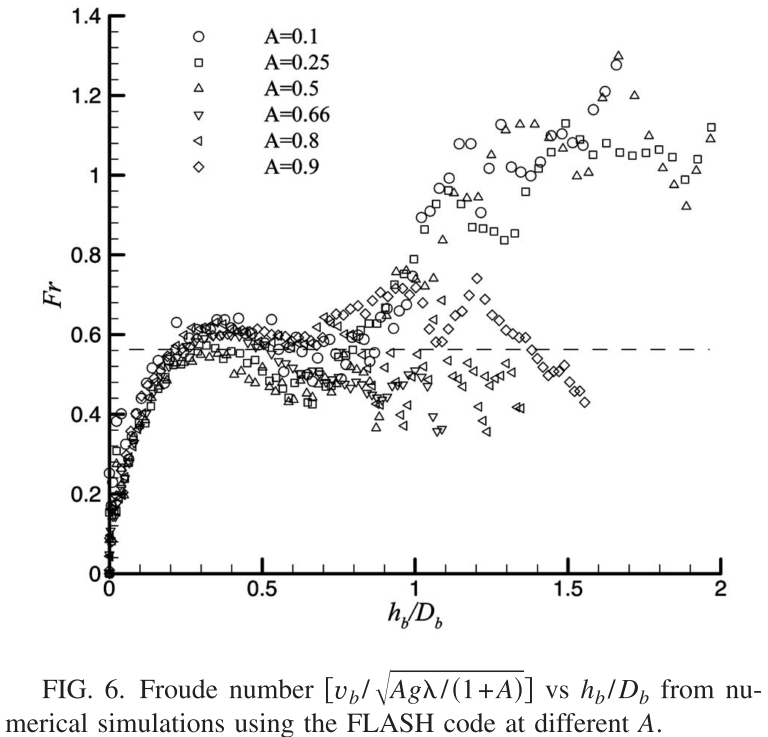
\includegraphics[height=0.5\textheight]{graphics/fr_flash.png}
~~~~
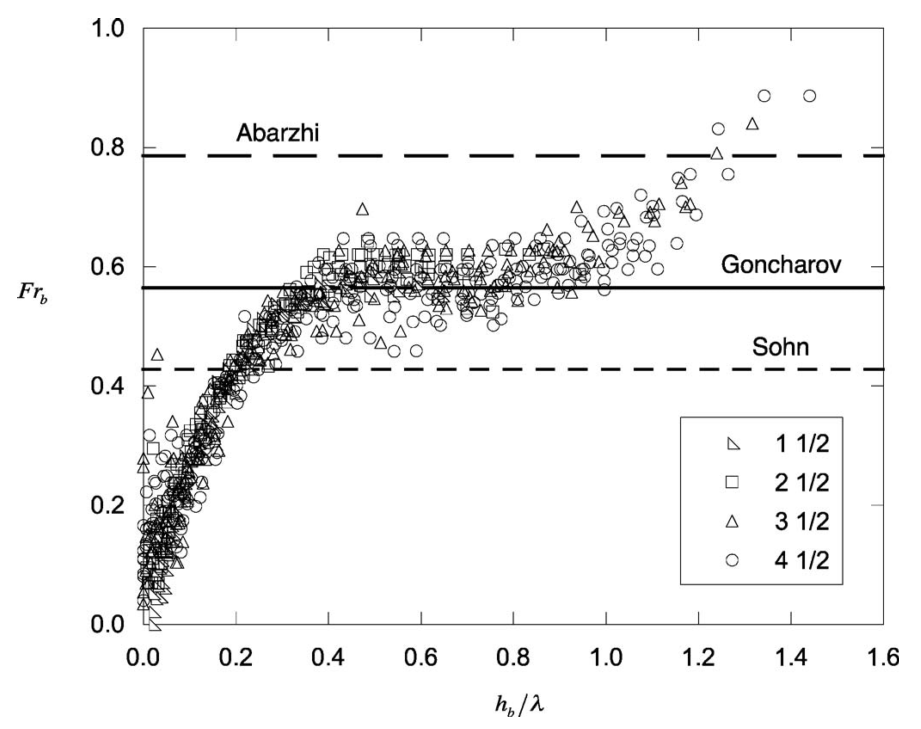
\includegraphics[height=0.5\textheight]{graphics/wilkinson_Fr.png}

{\footnotesize Simulations by Ramaprabhu and Dimonte, experiments by Wilkinson and Jacobs.}
}

\end{frame}

%===============================================================%
\section{Hypothesis}
%===============================================================%


\begin{frame}
Potential flow models assume no vorticity generation at the boundary,
which doesn't make sense for low-Atwood flows.

\vspace{20pt} \pause
Let's focus on buoyancy-drag instead:
\begin{equation*}
(\rho_1 + \rho_2) \mathcal{V} \ddot{h} = (\rho_2 - \rho_1) \mathcal{V} g - C \rho \dot{h}^2 \mathcal{A},
\end{equation*}
where $h$ is the bubble height, $\mathcal{V}, \mathcal{A}$ are characteristic volumes and areas, resp, and $C$ is a drag coefficient.

\vspace{20pt} \pause
For the single-mode RTI, $\mathcal{V} \sim \lambda^2 h$ and $\mathcal{A} \sim \lambda^2$, so:
\begin{equation*}
\dot{h}\left[\ddot{h} == 0\right] \sim \sqrt{h}
\end{equation*}
There is no terminal velocity at all!

\end{frame}


\begin{frame}
To balance the buoyancy, we add a viscous drag term:
\begin{equation*}
F_\nu \sim C \nu h \dot{h},
\end{equation*}
which is linear in $h$ so it can balance the buoyancy.
\begin{equation*}
\dot{h}\left[\ddot{h} == 0\right] = \frac{A g \lambda^2}{C \nu}
\end{equation*}
\pause

The growth is still terminal, but generally at a greater bubble velocity than predicted by inviscid potential flow models.
\vspace{20pt} \pause

Let's build this idea into a full model.
\end{frame}

\begin{frame}
Write down the forces and inertias with undetermined coefficients.
\begin{align*}
\text{Force} &= \overbrace{C_0 A g \lambda^2 h}^{\text{buoyancy}} - \overbrace{C_1 \lambda^2 \dot{h}^2}^{\text{form drag}} - \overbrace{C_2 \nu h \dot{h}}^{\text{skin drag}} \\
\text{Inertia} &= \underbrace{C_3 \lambda^2 h}_{\text{cylinder}} + \underbrace{C_4 \lambda^3}_{\text{sphere}}
\end{align*}\pause

We can drop $C_0$ and simplify:
\begin{equation*}
\ddot{h} = \frac{A g h - C_1 \dot{h^2} - C_2 \nu (h/\lambda^2) \dot{h}}{C_3 h + C_4 \lambda}
\end{equation*}
which has an asymptotic terminal velocity:
\begin{equation*}
\dot{h} = \frac{A g \lambda^2}{C_2 \nu}
\end{equation*}\pause
This is a problem: mixing.
\end{frame}

\begin{frame}
If $\dot{h}$ is bounded, mixing ultimately dominates the inflow of pure fluid.
\begin{equation*}
\frac{d V_p}{dt} \sim \lambda^2 \dot{h} - D h 
\end{equation*}
\pause

We'll track the volume of mixed fluid instead, $V_m \equiv M$, and define the effective Atwood number wrt the volume fraction of mixed fluid:
\begin{equation*}
A = A_0 \left(1 - \frac{M}{V}\right)
\end{equation*}
where $A_0$ is the Atwood number of pure fluids.
\vspace{20pt} \pause

Now we need a model for $M$, but we can check it directly.
\end{frame}

\begin{frame}
Assume the bubble has two parallel diffusive planar interfaces:
\begin{equation*}
\phi_{1D}(r) \sim \text{erf}\left[\frac{r}{\delta}\right] - \text{erf}\left[\frac{r - d}{\delta}\right]
\end{equation*}
where $\phi_{1D}$ is the 1D mass profile, $\delta$ is the interface width, and $d$ is the bubble diameter.
\vspace{20pt}\pause

Integrating and multiplying by a surface area term:
\begin{equation*}
M \approx \overbrace{\left(C_5 \lambda h + C_6 \lambda^2\right)}^{\text{surface area}} \overbrace{\left[\frac{2 \delta}{\sqrt{\pi}} \left(1 - e^{-d^2 / \delta^2}\right) + 2 d \left(1 - \text{erf}\left[\frac{d}{\delta}\right]\right)\right]}^{\text{1D mixing}}
\end{equation*}
with $d = C_5 \lambda / 8$, $\delta = 2 \sqrt{D t}$, and a generic volume:
\begin{equation*}
V = C_7 \lambda^2 h + C_8 \lambda^3
\end{equation*}
\end{frame}

\begin{frame}
We can constrain 3 parameters by fitting limits:
\begin{itemize}
  \item $C_4 = (2 \pi)^{-1}$ from the inviscid immiscible linear theory
  \item $C_6 = 1$ from matching the initial condition
  \item $C_8 = \pi^{-1}$ from the miscible linear theory
\end{itemize}

We can estimate the rest by physical argument:
\begin{itemize}
  \item $C_1$ from known drag coefficients
  \item $C_2$ from Poiseuille flow
  \item $C_3, C_7$ should be about 1
  \item $C_5$ should be about $\pi$
\end{itemize}
\end{frame}

\begin{frame}
\textbf{Hypothesis:} this model captures the dynamics of the low-Atwood single-mode Rayleigh-Taylor instability in cases when the bubble has a steady structure, i.e. moderate Grashof number (square of Reynolds number).
\end{frame}

%===============================================================%
\section{Methods}
%===============================================================%

\begin{frame}
Experiments are \textit{hard}, so we use direct numerical simulations
of the incompressible Navier-Stokes equations.
\begin{itemize}
  \item Very high order spectral elements
  \item Specially tailored version of Nek5000 (NekBox)
\end{itemize}
\vspace{20pt}\pause

Two important qualifications of the methods:
\begin{enumerate}
  \item They include all relevant physical processes (validation)
  \item They are cheap and accurate enough to do a parameter sweep (performance, convergence)
\end{enumerate}
\end{frame}

\begin{frame}
I validated NekBox against single-mode RTI experimental results of Wilkinson and Jacobs.
Submitted to \textit{Physical Review Fluids.}
\begin{center}
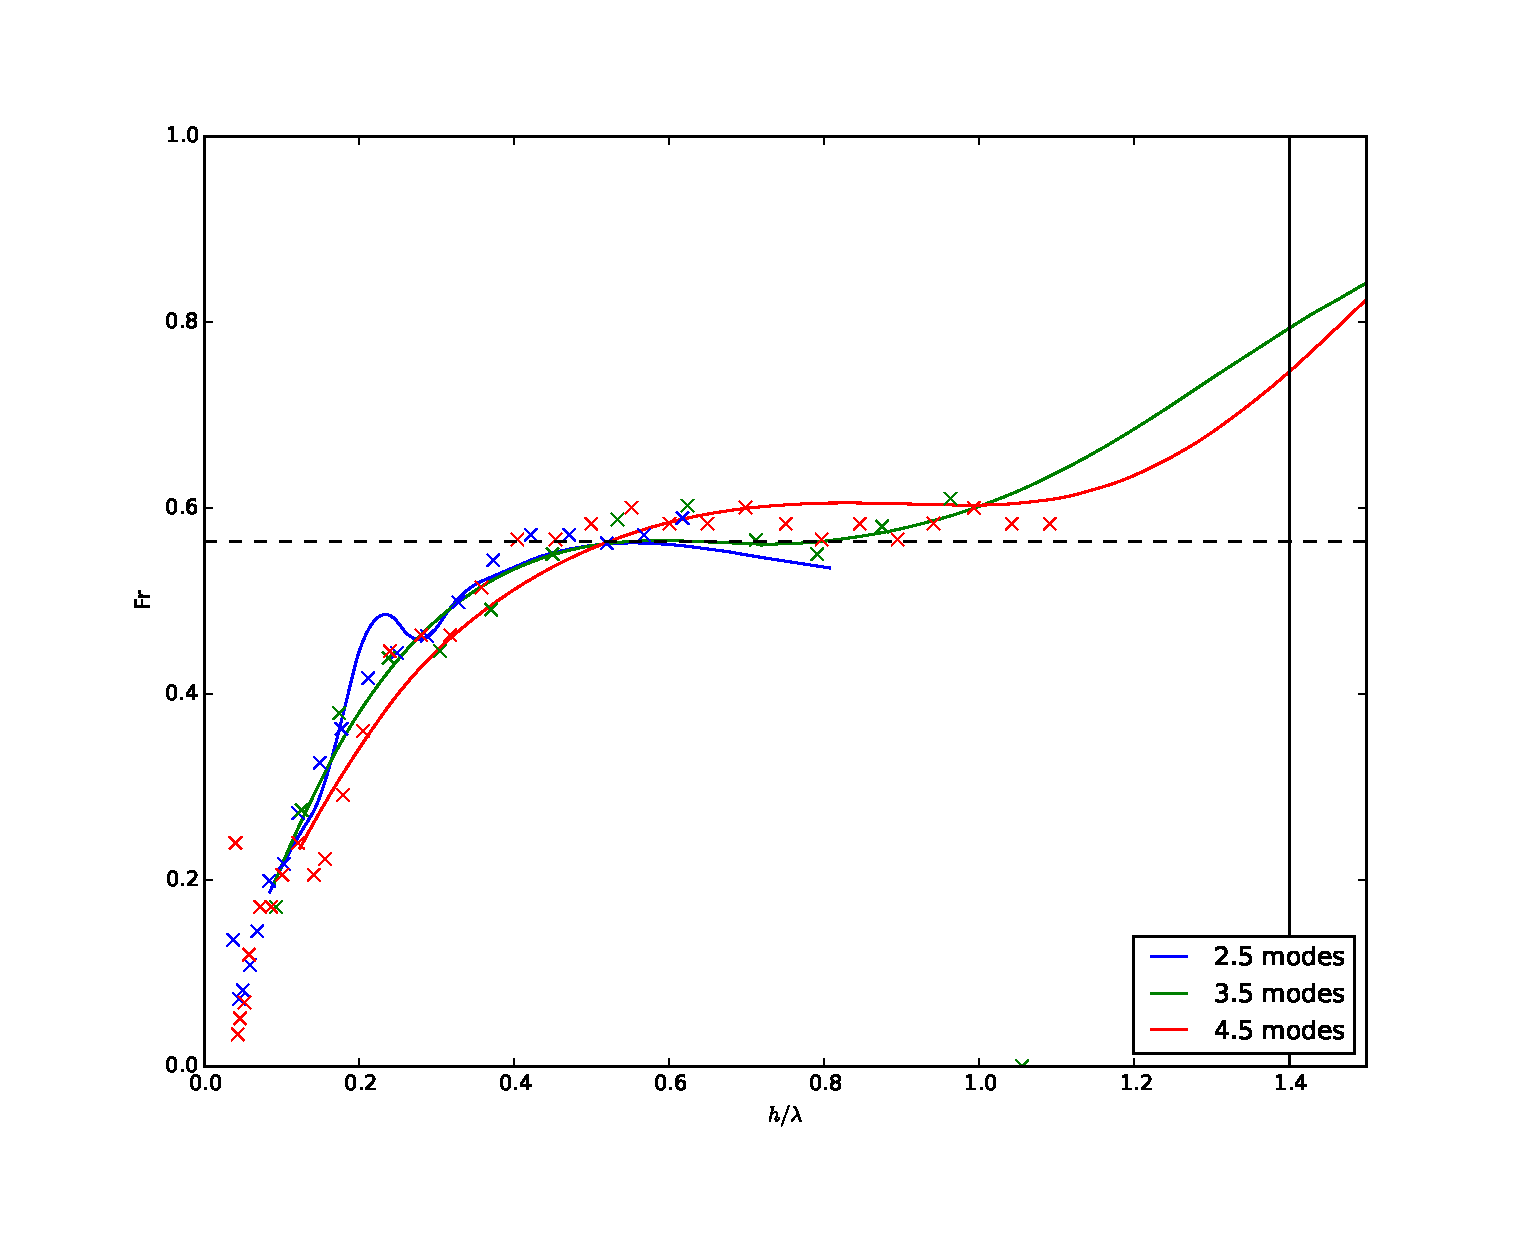
\includegraphics[height=0.9\textheight]{graphics/Fr.eps}
\end{center}
\end{frame}

\begin{frame}
I performed an accuracy/cost/convergence study for a typical point in the parameter sweep.
Accepted to International Supercomputing.
\begin{center}
\vspace{-10pt}
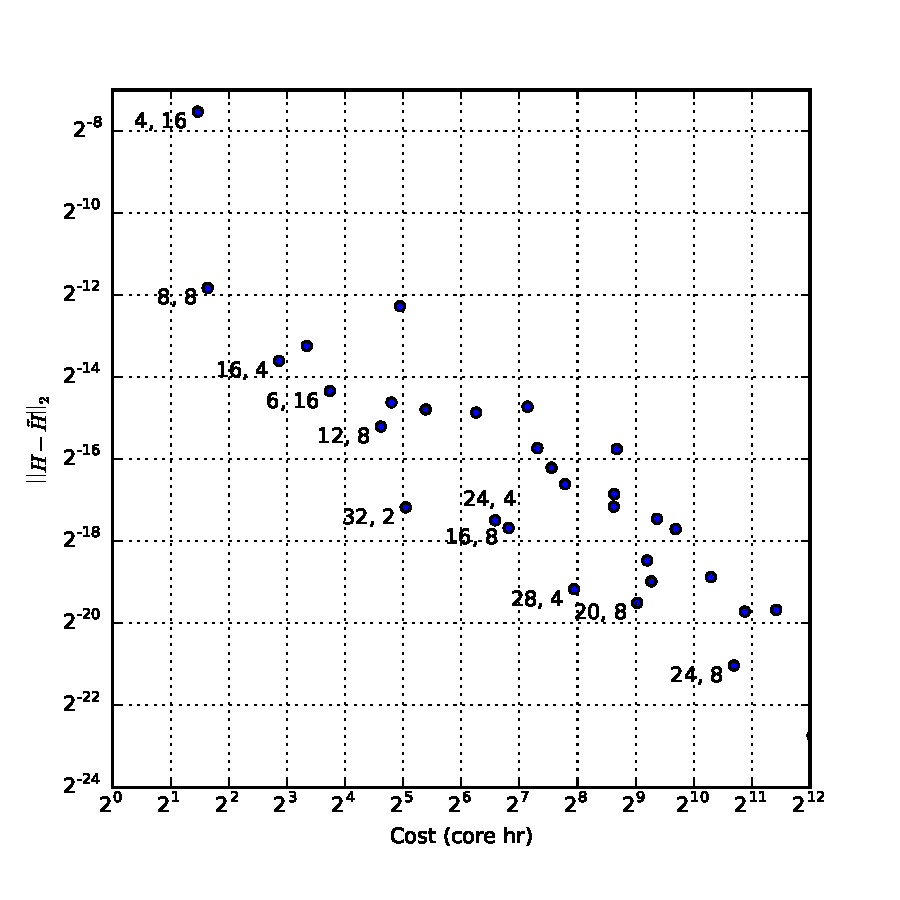
\includegraphics[height=0.75\textheight]{graphics/mira_H.pdf}
\end{center}
\vspace{-20pt}
Improved usage made calculations $16\times$ faster, optimization was another $20\times$.
\end{frame}

%===============================================================%
\section{Experiment}
%===============================================================%

\begin{frame}
Sampled Grashof numbers from $10^2$ to $10^6$ and Schmidt number $1$ to $10^2$.
\begin{itemize}
  \item 28 distinct simulations
\end{itemize}
\vspace{10pt} \pause

Highest quality simulations to date:
\begin{itemize}
  \item Relative error in bubble height less than $0.01\%$
  \item Domain height of $22\lambda$ (vs $6\lambda$)
\end{itemize}
\vspace{10pt} \pause

Flow simulated until either:
\begin{itemize}
  \item Bubble stops rising (success)
  \item Bubble reaches $3/4$ domain height (need bigger simulation)
\end{itemize}
\end{frame}

\begin{frame}
The 1-parameter mixing model is fit first, using the true bubble height as input.
\begin{itemize}
  \item Prevents over-fitting
  \item Non-linear fit with basin-hopping/sequential-least-squares
\end{itemize}
\vspace{20pt} \pause

The 4-parameter dynamics model is fit given the mixing model.
\begin{itemize}
  \item Non-linear fit with covariance matrix assisted evolution strategy
  \item Mixing model used to get cancellation of errors
  \item Constraints set by physical argument, e.g. $C_3 \ge 1$.
  \item Polished with sequential-least-squares
\end{itemize}
\end{frame}

%===============================================================%
\section{Results}
%===============================================================%
\begin{frame}[t]
The model is very accurate for the bubble height and reasonably accurate for the mixed volume.
\begin{center}
\only<2>{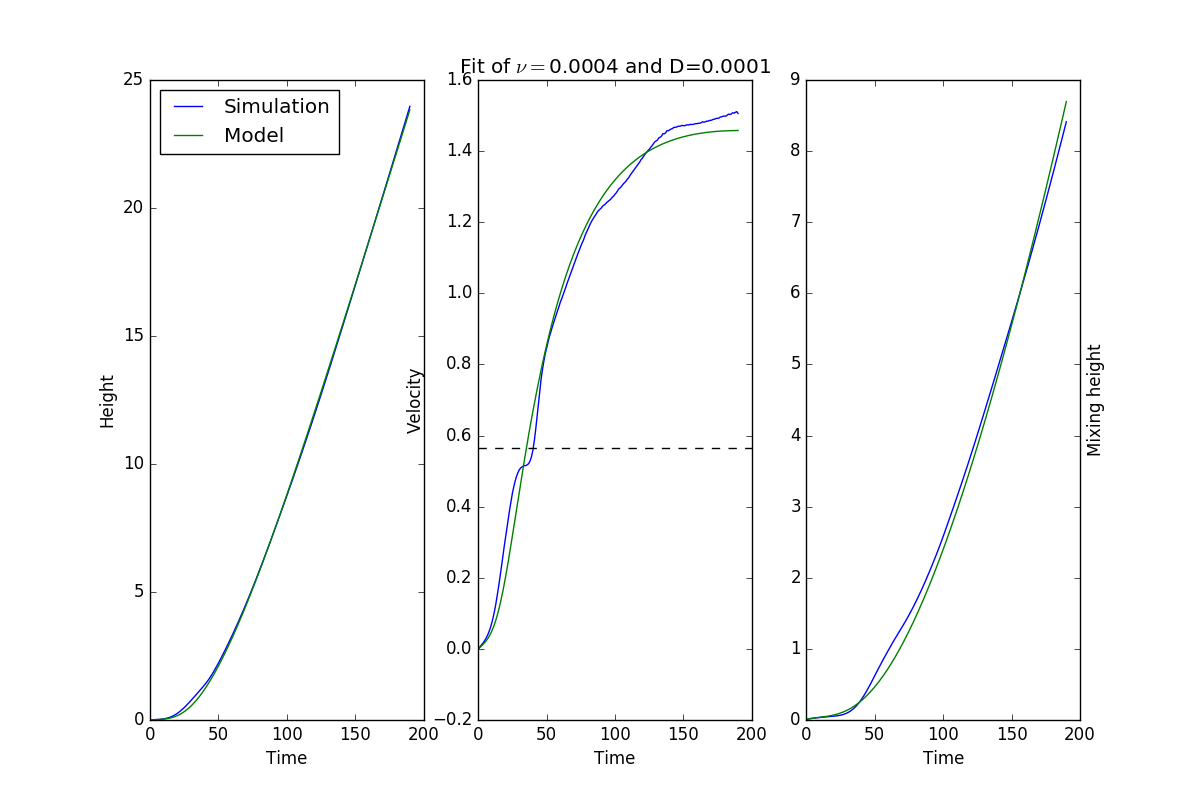
\includegraphics[width=0.95\textwidth]{graphics/H-4-1.png}}
\only<3>{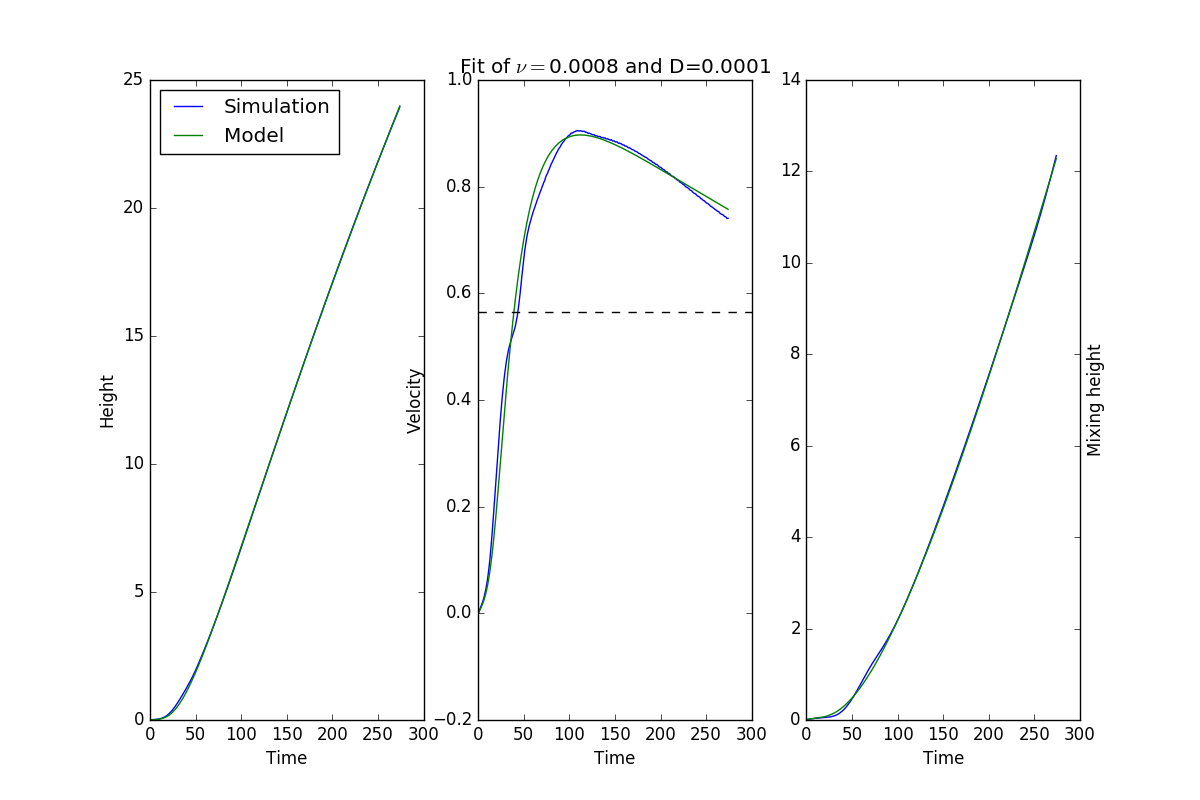
\includegraphics[width=0.95\textwidth]{graphics/H-8-1.png}}
\only<4>{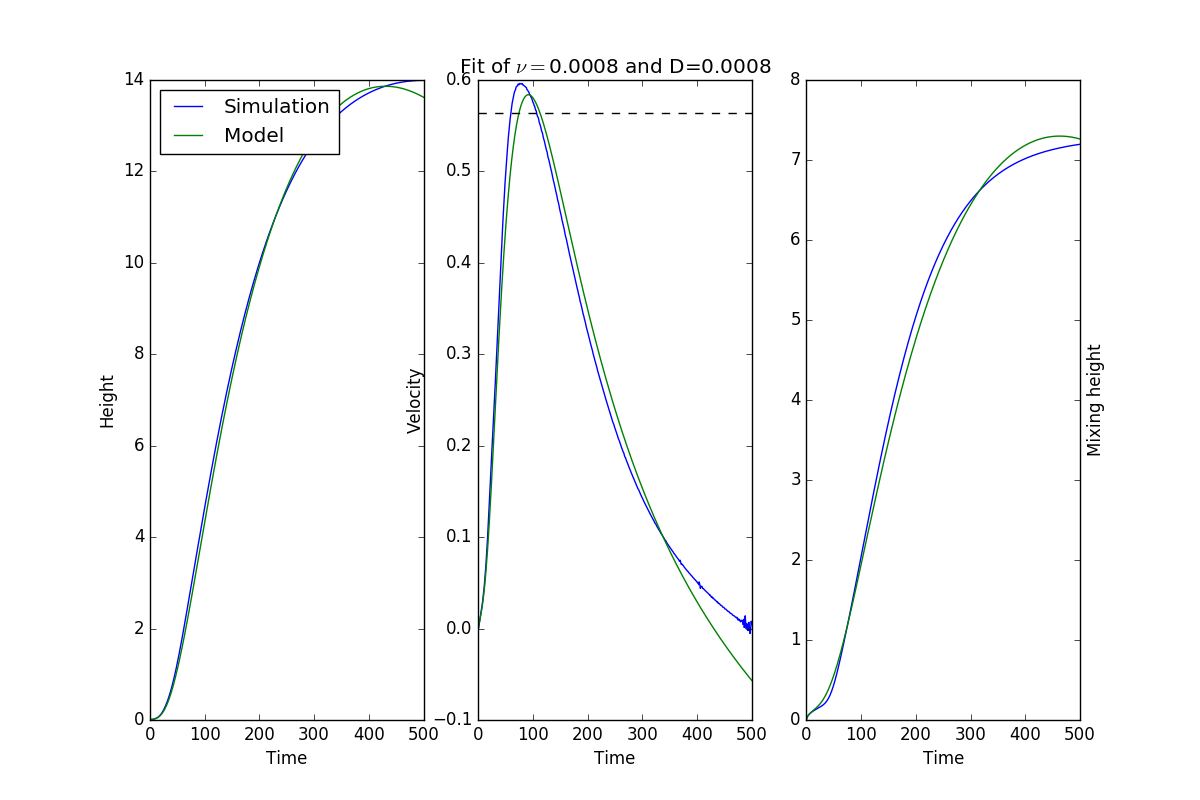
\includegraphics[width=0.95\textwidth]{graphics/H-8-8.png}}
\only<5>{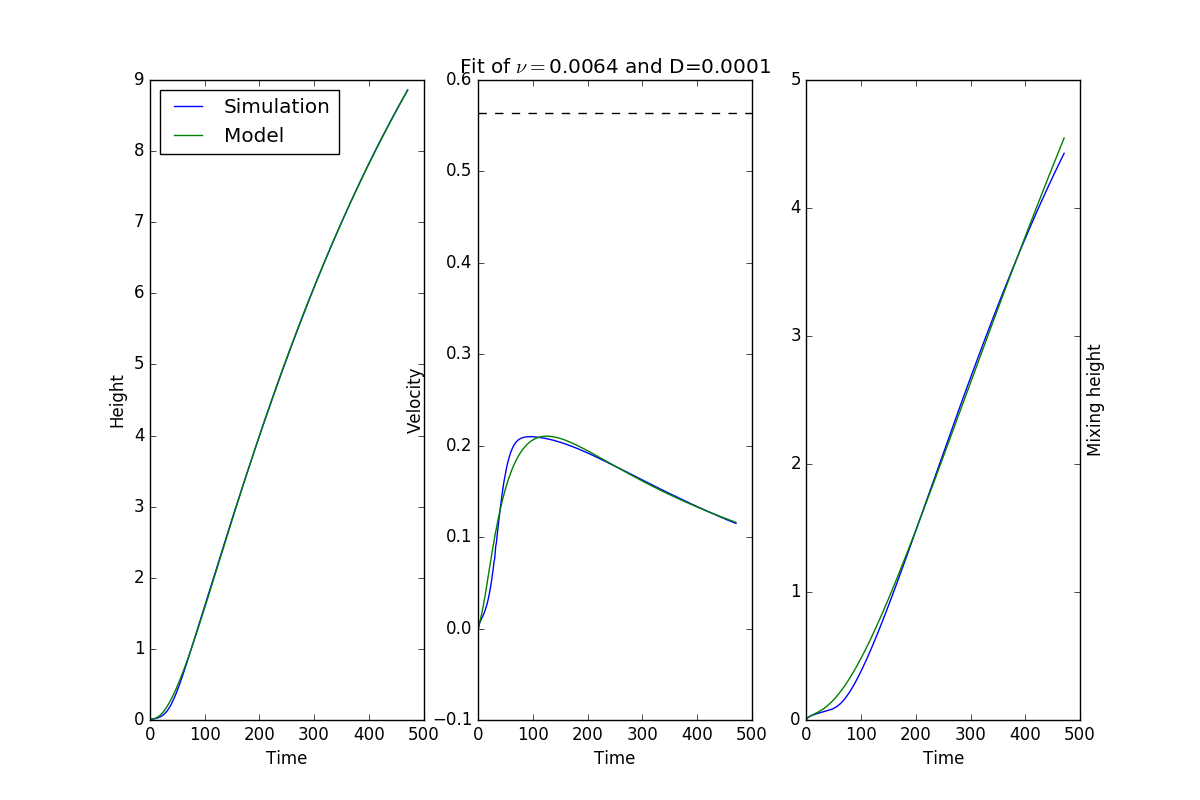
\includegraphics[width=0.95\textwidth]{graphics/H-64-1.png}}
\end{center}
\end{frame}

\begin{frame}[t]
Let's define some numbers:
\begin{equation*}
\text{Gr} = \frac{A g \lambda^3}{\nu^2} \qquad \text{Sc} = \frac{\nu}{D} \qquad \text{Ra} = \text{Gr} \text{Sc} = \frac{A g \lambda^3}{\nu D}
\end{equation*}

At early times, we can ignore viscosity and diffusion:
\begin{equation*}
\tau \sim \sqrt{\frac{\lambda}{A g}} \qquad \tilde{v} \sim \sqrt{A g \lambda}
\end{equation*}

At later times, we can't
\begin{equation*}
\tau \sim \frac{\nu}{A g \lambda} \qquad \tilde{v} \sim \frac{A g \lambda}{\nu} \qquad \frac{\delta}{\lambda} \sim \sqrt{\frac{D \tau}{\lambda^2}} = \sqrt{\frac{1}{\text{Ra}}}
\end{equation*}
\end{frame}

\begin{frame}[t]
There is less error at higher Grashof, Schmidt numbers.
\begin{center}
\only<1>{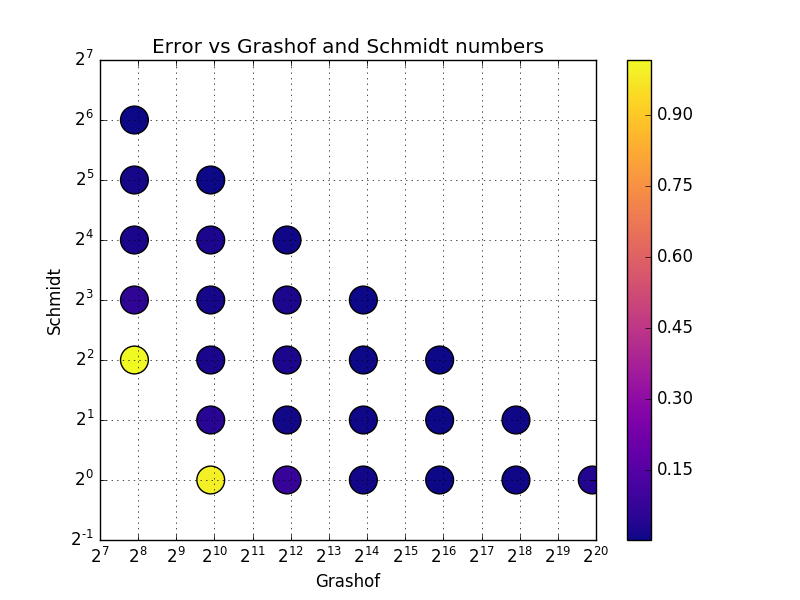
\includegraphics[width=0.8\textwidth]{graphics/Error-vs-Grashof-Schmidt.png}}
\only<2>{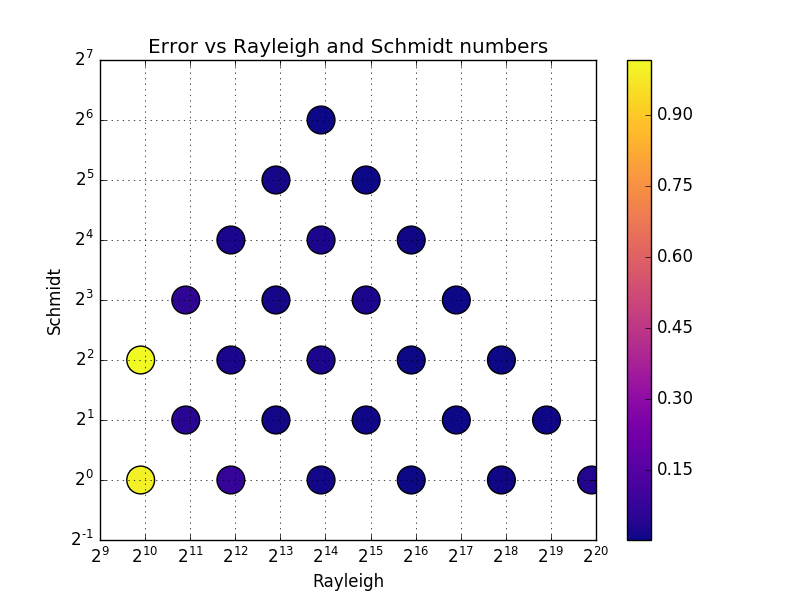
\includegraphics[width=0.8\textwidth]{graphics/Error-vs-Rayleigh-Schmidt.png}}
\end{center}
\end{frame}

\begin{frame}[t]
$C_1$ generally increases with Rayleigh number.
\begin{center}
\only<1>{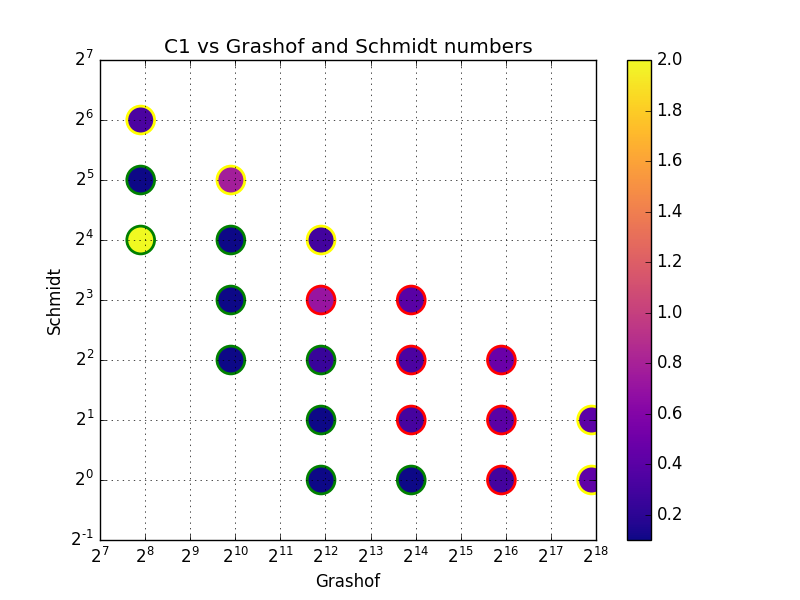
\includegraphics[width=0.8\textwidth]{graphics/C1-vs-Grashof-Schmidt.png}}
\only<2>{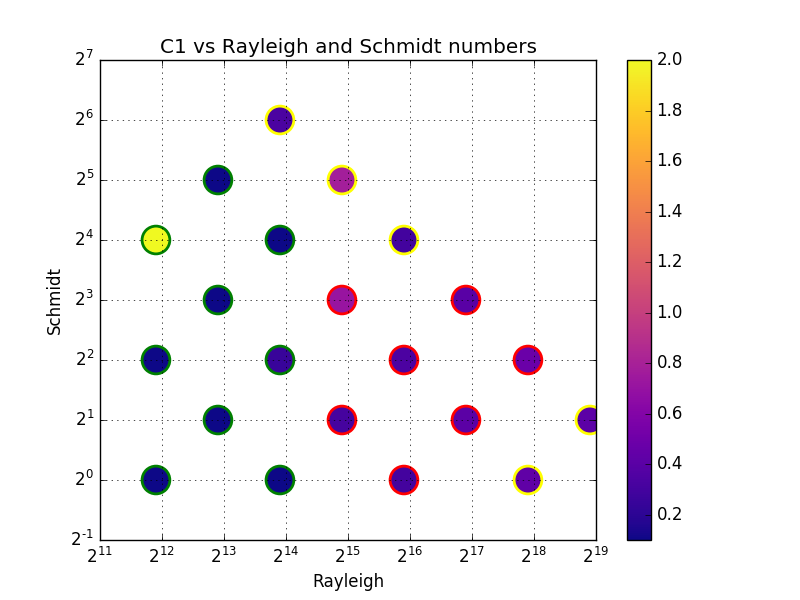
\includegraphics[width=0.8\textwidth]{graphics/C1-vs-Rayleigh-Schmidt.png}}
\end{center}
\end{frame}

\begin{frame}[t]
$C_2$ generally increases with Rayleigh number.
\begin{center}
\only<1>{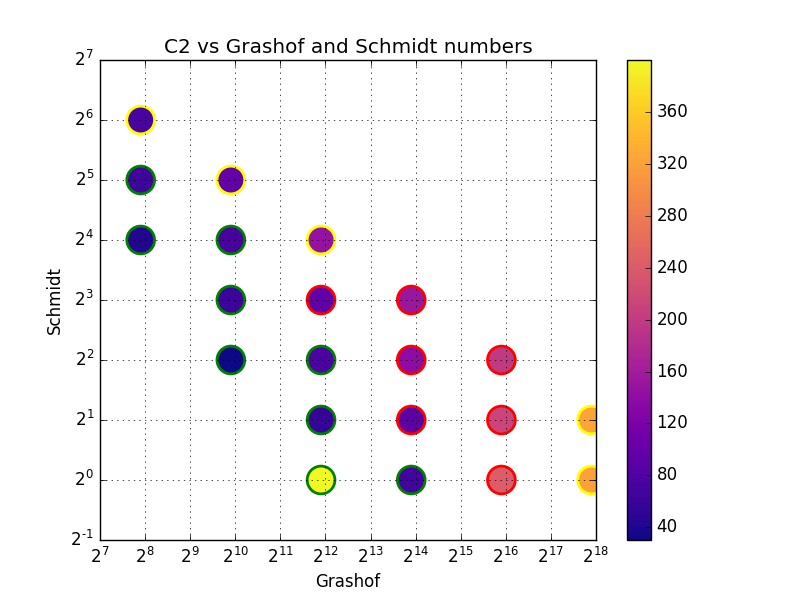
\includegraphics[width=0.8\textwidth]{graphics/C2-vs-Grashof-Schmidt.png}}
\only<2>{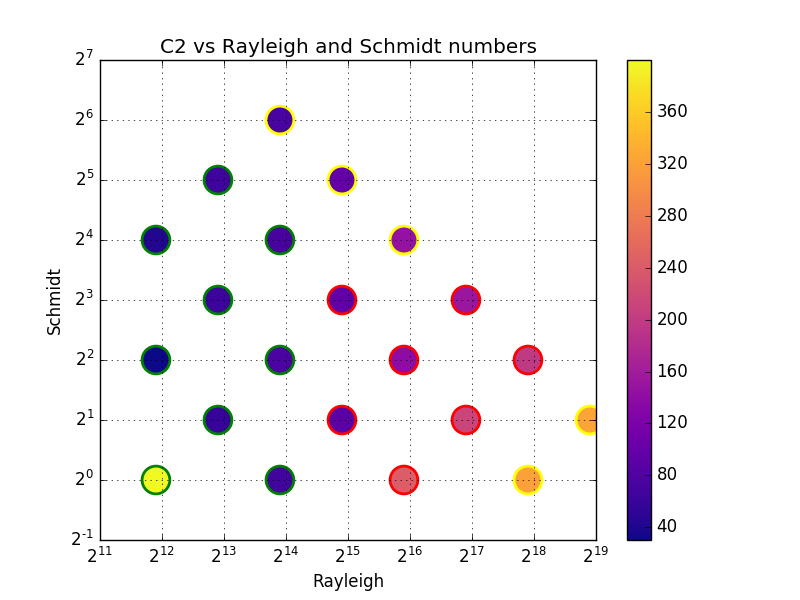
\includegraphics[width=0.8\textwidth]{graphics/C2-vs-Rayleigh-Schmidt.png}}
\end{center}
\end{frame}

\begin{frame}[t]
$C_3$ is under-constrained at low Grashof number.
\begin{center}
\only<1>{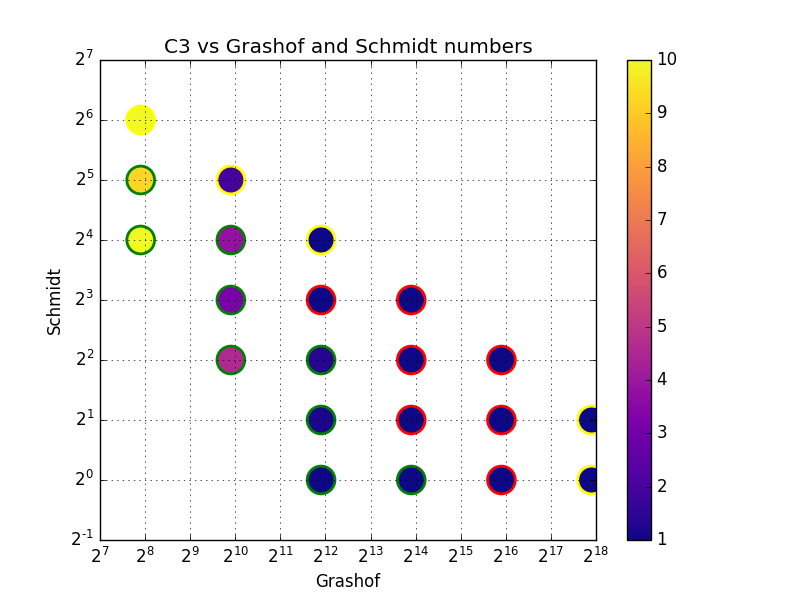
\includegraphics[width=0.8\textwidth]{graphics/C3-vs-Grashof-Schmidt.png}}
\only<2>{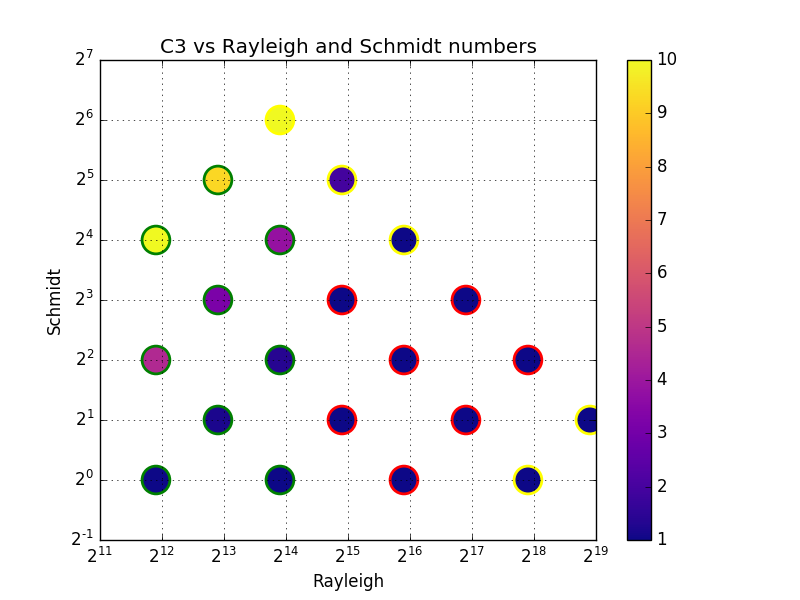
\includegraphics[width=0.8\textwidth]{graphics/C3-vs-Rayleigh-Schmidt.png}}
\end{center}
\end{frame}

\begin{frame}[t]
$C_5$ decreases with diffusivity.
\begin{center}
\only<1>{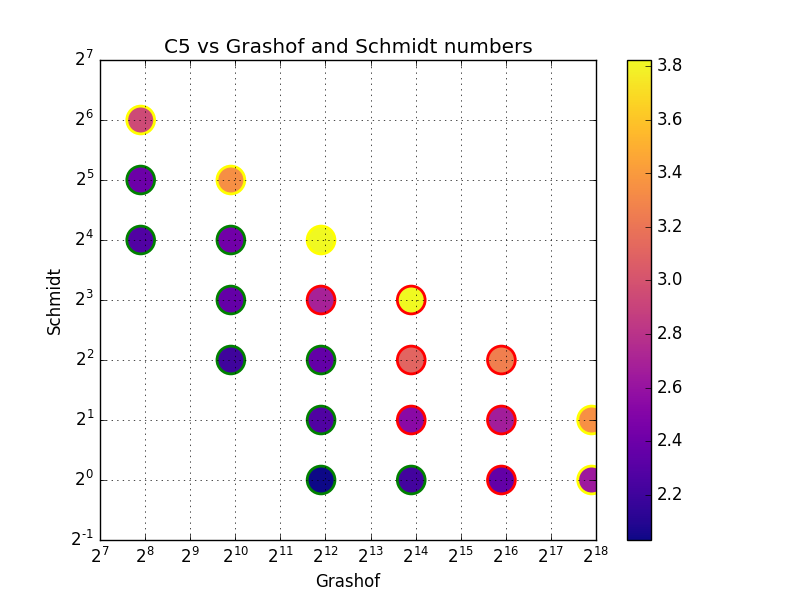
\includegraphics[width=0.8\textwidth]{graphics/C5-vs-Grashof-Schmidt.png}}
\only<2>{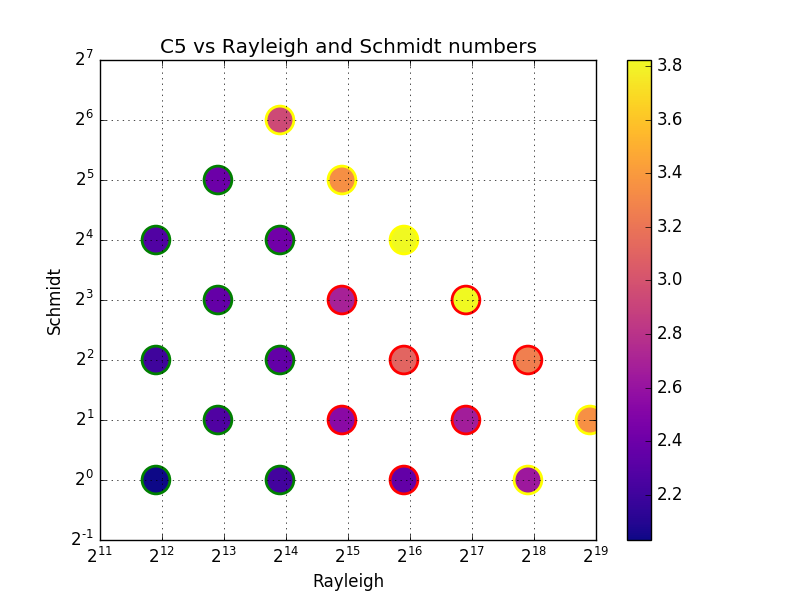
\includegraphics[width=0.8\textwidth]{graphics/C5-vs-Rayleigh-Schmidt.png}}
\end{center}
\end{frame}

\begin{frame}[t]
$C_7$ is about 1, except for a few breaks.
\begin{center}
\only<1>{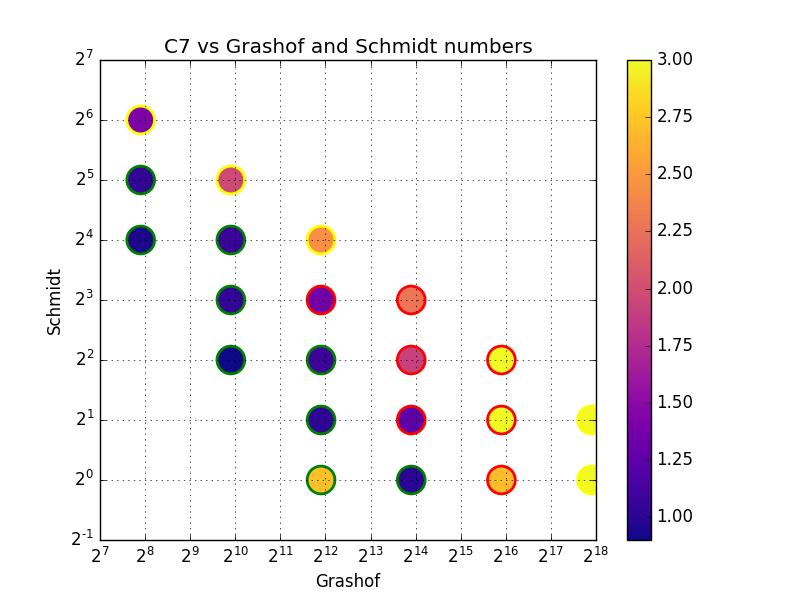
\includegraphics[width=0.8\textwidth]{graphics/C7-vs-Grashof-Schmidt.png}}
\only<2>{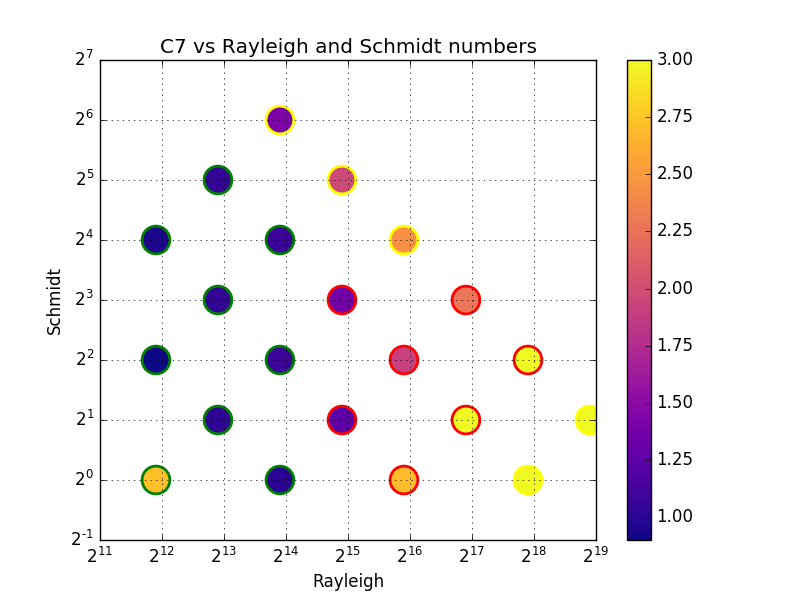
\includegraphics[width=0.8\textwidth]{graphics/C7-vs-Rayleigh-Schmidt.png}}
\end{center}
\end{frame}

%===============================================================%
\section{Conclusions}
%===============================================================%
\begin{frame}
We have identified the features of low-Atwood single mode flows
\begin{itemize}
  \item The only late-time velocity is viscous
  \item Any finite viscosity and diffusivity results in mixing death
  \item \textit{Re-acceleration} is a moderate-time transient
\end{itemize}
\vspace{10pt} \pause

The proposed model is quantitatively descriptive
\begin{itemize}
  \item Depends only on initial conditions
  \item Low error rates over a range of Grashof and Schmidt numbers
  \item Admits physical interpretation of parameters
\end{itemize}
\end{frame}

\appendix
%===============================================================%
\section*{Thesis}
%===============================================================%
\begin{frame}{Organization of thesis}

\resizebox{\textwidth}{!}{
\tikzstyle{block} = [rectangle, draw, 
    text width=10em, text centered, rounded corners, minimum height=10em]
\tikzstyle{intro} = [block, fill=blue!20]  
\tikzstyle{model} = [block, fill=yellow!20] 
\tikzstyle{valid} = [block, fill=black!30!green] 
\tikzstyle{optim} = [block, fill=black!50!green] 
\tikzstyle{other} = [block, fill=black!10!purple] 
\tikzstyle{sloud} = [draw, star,fill=green!20, minimum height=2em]
\tikzstyle{ar}    = [->, thick, shorten <=8pt, shorten >=8pt]
\tikzstyle{wlock} = [rectangle, draw, 
    text width=5em, text centered, minimum height=4em]


\begin{tikzpicture}[node distance=5cm, auto]
\node[intro] (layzer) {Potential flow models of Layzer and Goncharov};
\node[intro, right of=layzer] (wilk) {Single mode experiments by Wilkinson};
\node[model, right of=wilk] (bdm) {Buoyancy-drag model with viscosity};
\node[model, right of=bdm, node distance=8cm] (param) {Model parameters and accuracy};
\node[model, right of=param] (behavior) {Model behavior};
\node[model, right of=behavior] (ques) {Open questions};

\node[valid, below of=bdm, node distance=8cm] (val) {Validation against Wilkinson's experiments};
\node[valid, left of=val] (sim) {Simulation with spectral element method};
\node[valid, left of=sim] (NS) {Incompressible Navier-Stokes};
\node[optim, right of=val] (conv) {Convergence \& performance study};
\node[optim, right of=conv] (tuning) {Tuning for efficiency};
\node[optim, right of=tuning] (data) {Simulation of data set};

\node[other, below of=sim] (ts) {Mixed order time-steppers};
\node[other, below of=tuning] (xsmm) {LIBXSMM etc.};
\node[other, below of=data] (dask) {DAG-based workflows in nekpy with dask};
\node[other, below of=conv] (proj) {Subspace projection for successive RHS};

\path (layzer) edge[ar] (wilk);
\path (wilk) edge[ar] (bdm);
\path (bdm) edge[ar, dotted] node {Hard analytically} (param);
\path (param) edge[ar] (behavior);
\path (behavior) edge[ar] (ques);

\path (NS) edge[ar] (sim);
\path (sim) edge[ar] (val);
\path (val) edge[ar] (conv);
\path (conv) edge[ar] (tuning);
\path (tuning) edge[ar] (data);

\path (bdm) edge[ar, out=270, in=90] (NS);
\path (data) edge[ar, out=90, in=270] (param);

\path (ts) edge[ar, dotted] (sim);
\path (xsmm) edge[ar, dotted] (tuning);
\path (dask) edge[ar, dotted] (data);
\path (proj) edge[ar, dotted] (conv);

%\path () edge[ar] ();
%\path () edge[ar] ();

%\path (ibc) edge[ar, bend right=45] (pet);
%\path (inp) edge[ar, bend right=45] (pet);
%\path (raw) edge[ar, bend left=45] (pet);
%\path (opp) edge[ar, bend left=45] (pet);

\end{tikzpicture}
}
\end{frame}

%===============================================================% 
\end{document}
%===============================================================%
